\chapter{Einleitung}

Autonome Fahrzeuge zählen zu den bedeutendsten technologischen Entwicklungen im Bereich der Mobilität unserer Zeit. Angetrieben durch Fortschritte in den Bereichen Sensorik, künstliche Intelligenz und Fahrzeugarchitektur ist absehbar, dass autonome Fahrfunktionen zunehmend in Serienfahrzeuge integriert werden. Dabei spielen vielfältige gesellschaftliche und ökonomische Faktoren eine Rolle: Neben dem demografischen Wandel und dem Fachkräftemangel im Transportsektor ist vor allem die fortschreitende Urbanisierung von zentraler Bedeutung. Mit der zunehmenden Konzentration der Bevölkerung in städtischen Räumen steigen sowohl das Verkehrsaufkommen als auch die Anforderungen an Sicherheit, Effizienz und Nachhaltigkeit im Mobilitätssystem. Laut einer Erhebung des United Nations Department of Economic and Social Affairs \cite{bpb2017} werden bis zum Jahr 2050 mehr als 50 \% der Menschen in den ökonomisch entwickelten Ländern in Städten leben. In Deutschland lag der Anteil der Stadtbevölkerung im Jahr 2015 bereits bei über 77 \% mit einer prognostizierten Steigerung auf 84,3 \% bis zum Jahr 2050. \cite{Statista2025}

\begin{center}
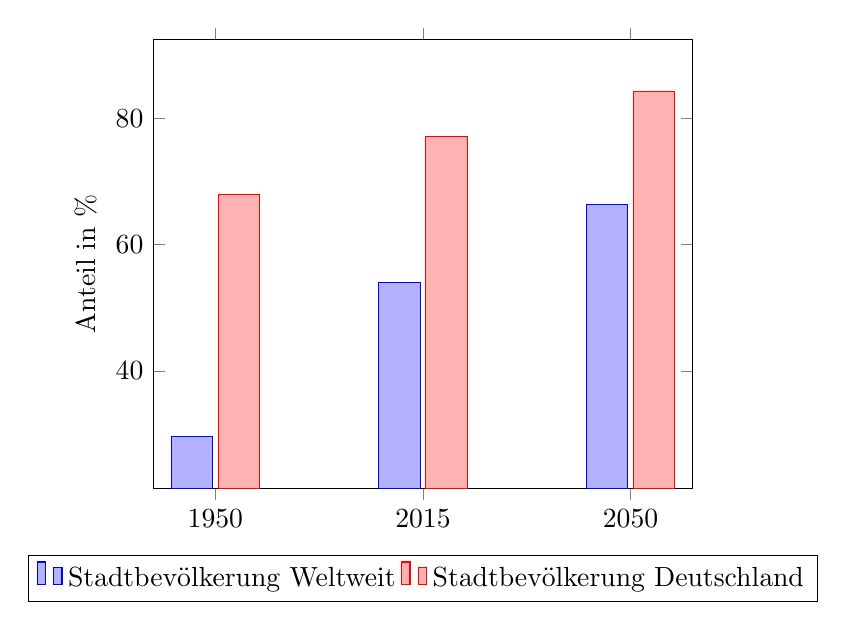
\begin{tikzpicture}
    \begin{axis}[
        ylabel=Anteil in \%,
        enlargelimits=0.15,
        legend style={at={(0.5,-0.15)},
            anchor=north,legend columns=-1},
        ybar,
        bar width=15pt,
        symbolic x coords={1950,2015,2050},
        xtick=data,
    ]
    \addplot coordinates {(1950,29.6) (2015,54) (2050,66.4)};
    \addplot coordinates {(1950,67.9) (2015,77.2) (2050,84.3)};

    \legend{Stadtbevölkerung Weltweit,Stadtbevölkerung Deutschland}
    \end{axis}
\end{tikzpicture}
\end{center}

Zugleich wird prognostiziert, dass die Gesamtbevölkerung von 7,3 Milliarden im Jahr 2015 auf 9,5 Milliarden im Jahr 2050 wachsen wird. In diesem Zusammenhang werden autonome Fahrzeuge als Schlüsseltechnologie betrachtet, da sie zur Reduzierung von Unfällen, zur Optimierung des Verkehrsflusses und zur besseren Auslastung vorhandener Infrastrukturen beitragen können. Prognosen zeigen, dass Fahrzeuge mit mindestens erweiterten teilautonomen Fahrfunktionen (Level 2+ oder höher) bis zum Jahr 2035 einen Marktanteil von 37\% erreichen werden. 

Mit der wachsenden Verbreitung solcher Fahrfunktionen steigen jedoch auch die Anforderungen an die zugrunde liegende Fahrzeugarchitektur. Durch die zunehmenden Integration künstlicher Intelligenz in autonome Fahrfunktionen steigen die Anforderungen an die Rechenleistung kontinuierlich. Moderne Algorithmen für Objekterkennung, Sensorfusion oder Entscheidungsfindung basieren auf tiefen neuronalen Netzen, deren Ausführung in Echtzeit enorme Rechenressourcen erfordert. Hinzu kommen weitere datenintensive Anwendungen wie hochauflösende Umgebungsmodellierung, V2X Kommunikation oder cloudgestützte Dienste, die zusätzliche Lasten erzeugen. Steuergeräte der neuesten Generation erreichen bereits heute Rechenleistungen im Bereich von mehreren hundert bis zu tausend Tera-OPS, was sie faktisch zu Hochleistungsrechnern im Fahrzeug macht. Diese Kapazitäten werden in der Praxis jedoch nicht jederzeit vollständig ausgeschöpft, da der Ressourcenbedarf stark von Fahrsituation und Funktionsumfang abhängt.

Vor diesem Hintergrund ergibt sich die Möglichkeit, ungenutzte Rechenleistung für externe Anwendungen bereitzustellen. In Smart-City-Szenarien könnten Fahrzeuge beispielsweise als dezentrale Knotenpunkte für die Verarbeitung von Sensordaten zur Verkehrssteuerung eingesetzt werden. Ebenso ließen sich flottenbasierte Optimierungsaufgaben wie Routenplanung oder Energieverbrauchsanalysen direkt auf den im Einsatz befindlichen Fahrzeugen ausführen. Darüber hinaus bietet sich die Nutzung für Edge-Computing-Dienste an, etwa zur Vorverarbeitung von Daten für Cloud-Plattformen oder zur Bereitstellung von Rechenressourcen für Dritte in der unmittelbaren Umgebung. Damit wandelt sich das Fahrzeug von einem rein konsumierenden Steuerungssystem zu einem aktiven Bestandteil verteilter Recheninfrastrukturen.

